% Holds, then snaps
% ---------------------------------------------------------------------------
% Skeleton only: section headings, figure includes and captions are in place;
% the bodies are deliberately empty and are written by hand.
%
% Build with:  python build_report.py
% ---------------------------------------------------------------------------

\documentclass[11pt,a4paper]{article}

\usepackage[T1]{fontenc}
\usepackage[utf8]{inputenc}
\usepackage{lmodern}
\usepackage[british]{babel}
\usepackage{microtype}

\usepackage[margin=3.2cm]{geometry}
\usepackage{graphicx}
\usepackage{booktabs}
\usepackage{amsmath}
\usepackage{siunitx}
\usepackage{caption}
\usepackage[hidelinks]{hyperref}
\usepackage[round,authoryear]{natbib}

\graphicspath{{../figures/}}
\captionsetup{font=small,labelfont=bf,width=0.92\textwidth}
\bibliographystyle{plainnat}

\newcommand{\eps}{\varepsilon}

% Every figure caption cites the file its numbers come from. See
% figures/MANIFEST.md for the full mapping.
\newcommand{\source}[1]{\par\smallskip\footnotesize\textit{Source:} \texttt{#1}}

\title{Holds, then snaps\\
\large When cooperation survives noise, and how it fails}
\author{Tarık Sahar}
\date{}

\begin{document}
\maketitle

\begin{abstract}
% TODO
\end{abstract}

\section{The question}
\label{sec:question}
% TODO

\section{Model and method}
\label{sec:method}

\subsection{The game}
\label{sec:game}
% TODO

\subsection{Strategies}
\label{sec:strategies}
% TODO

\subsection{Tournament}
\label{sec:tournament}
% TODO

\subsection{Replicator dynamics}
\label{sec:replicator}
% TODO

\subsection{Execution error and a stochastic horizon}
\label{sec:phasec-params}
% TODO

\subsection{Measuring cooperation from play, not from names}
\label{sec:metric}
% TODO

\section{The apparatus before noise}
\label{sec:apparatus}
% TODO

\begin{figure}[t]
  \centering
  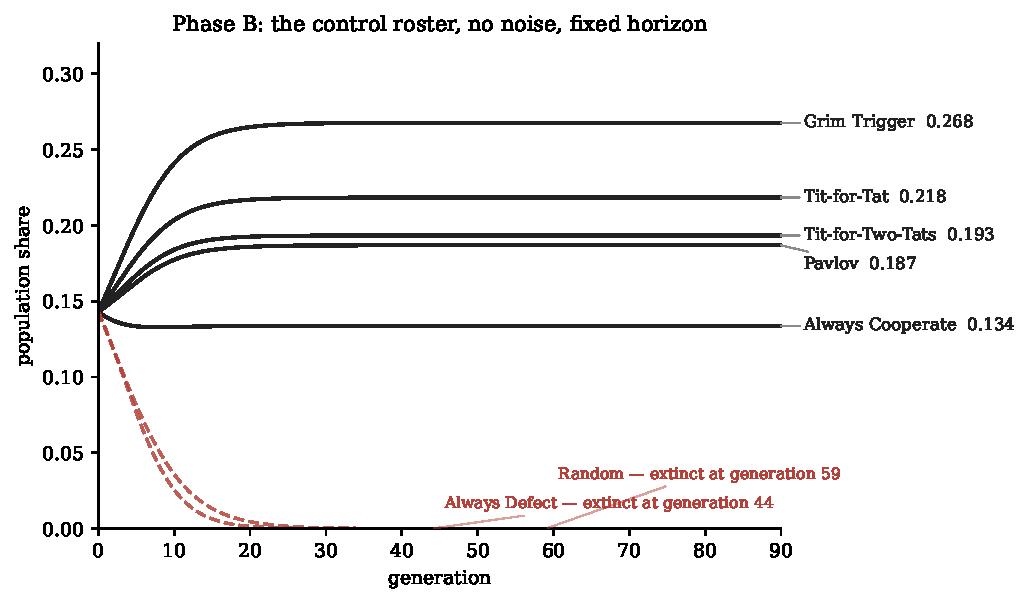
\includegraphics[width=\linewidth]{fig6_phase_b_trajectory.pdf}
  \caption{Replicator dynamics on the seven-strategy control roster with no
  execution error and a fixed horizon. Always Defect and Random are
  eliminated; the survivors are mutually neutral, so the final proportions
  record the transient rather than an equilibrium selection has chosen.
  \source{results/fig6\_phase\_b\_trajectory.csv}}
  \label{fig:phaseb}
\end{figure}

\section{The map}
\label{sec:map}
% TODO

\begin{figure}[t]
  \centering
  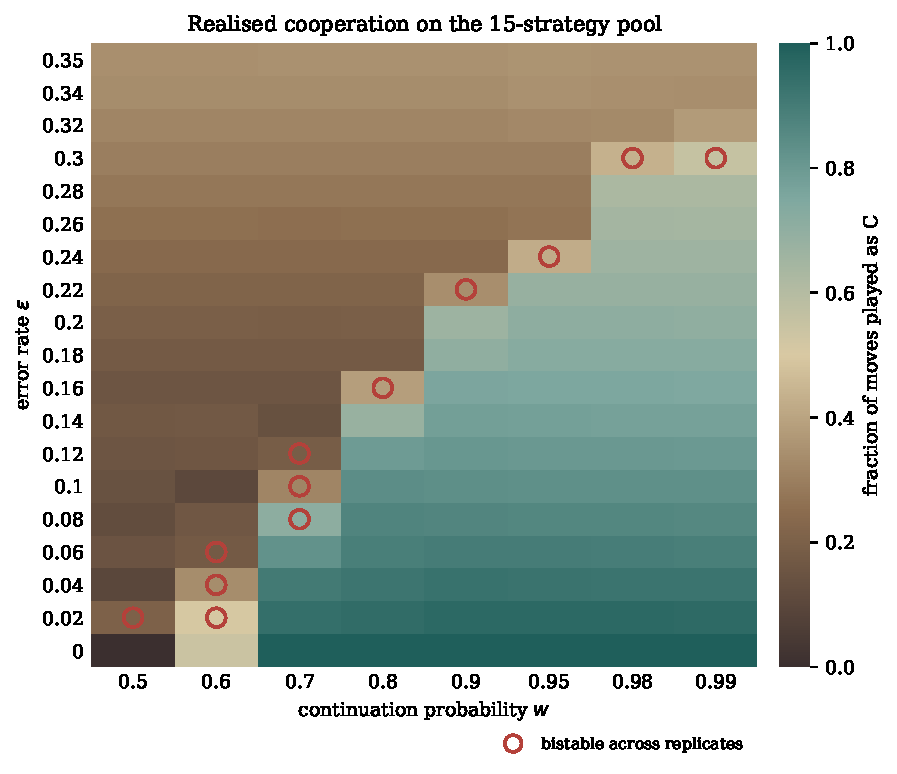
\includegraphics[width=0.92\linewidth]{fig1_map_pool.pdf}
  \caption{Realised cooperation across the error rate $\eps$ and the
  continuation probability $w$, on the fifteen-strategy pool. Colour is the
  fraction of moves actually played as \textsf{C}, averaged over five
  replicates. Ringed cells are bistable: replicates differing only in the
  tournament seed reach different attractors, and a mean describes neither.
  \source{results/fig1\_map\_pool.csv}}
  \label{fig:map}
\end{figure}

\subsection{The edge}
\label{sec:edge}
% TODO

\begin{figure}[t]
  \centering
  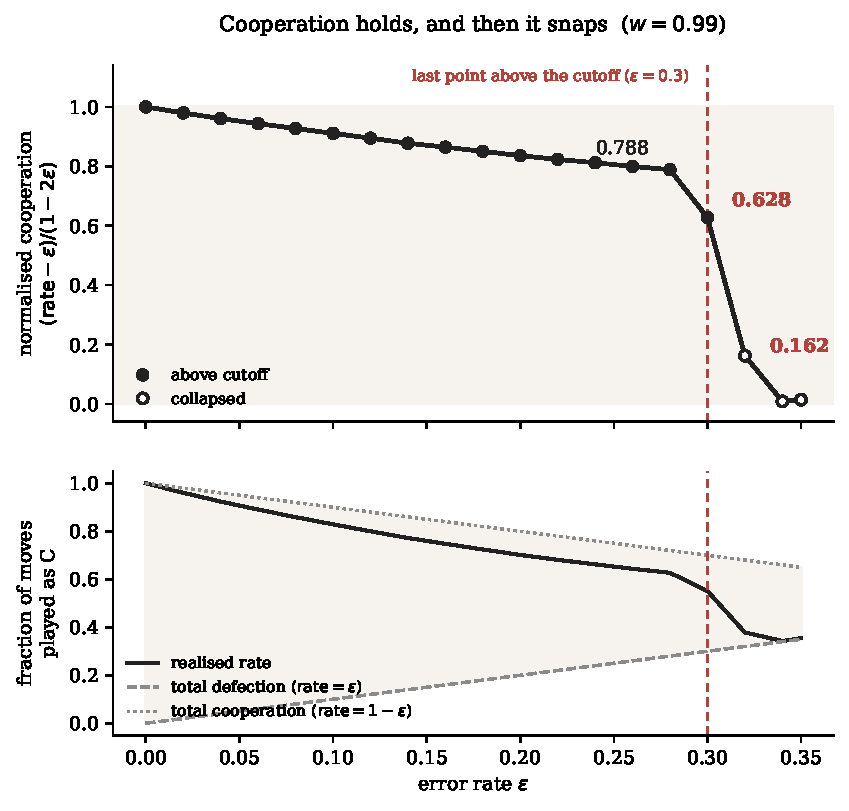
\includegraphics[width=0.92\linewidth]{fig2_edge_profile.pdf}
  \caption{The shape the report is named for, along the longest horizon
  ($w = 0.99$). Upper panel: cooperation normalised onto the band the error
  rate leaves available, $(\text{rate}-\eps)/(1-2\eps)$, so that $1$ is total
  cooperation and $0$ total defection at every $\eps$. It holds at $0.788$
  through $\eps = 0.28$, then falls to $0.628$ and $0.162$ over the next two
  grid steps. Lower panel: the raw rate against the two bounds it lies
  between; collapse is the rate meeting the lower one.
  \source{results/fig2\_edge\_profile.csv}}
  \label{fig:edge}
\end{figure}

\subsection{Two predictions, tested}
\label{sec:predictions}
% TODO

\section{The roster as a variable}
\label{sec:roster}
% TODO

\begin{figure}[t]
  \centering
  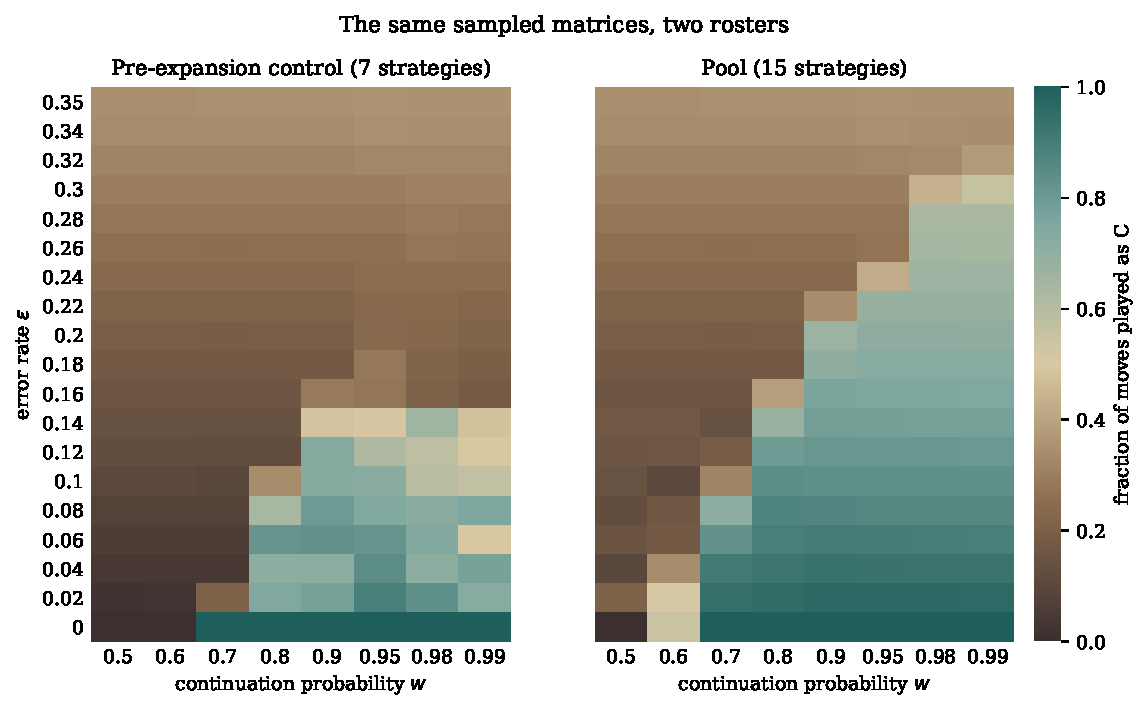
\includegraphics[width=\linewidth]{fig3_roster_comparison.pdf}
  \caption{The same sampled tournaments read twice: once over the seven
  strategies the earlier phases used, once over the fifteen-strategy pool.
  Because both maps are submatrices of one set of matrices, the difference
  between them cannot be sampling noise between two runs.
  \source{results/fig3\_roster\_comparison.csv}}
  \label{fig:rosters}
\end{figure}

\subsection{Sensitivity}
\label{sec:sensitivity}
% TODO

\begin{figure}[t]
  \centering
  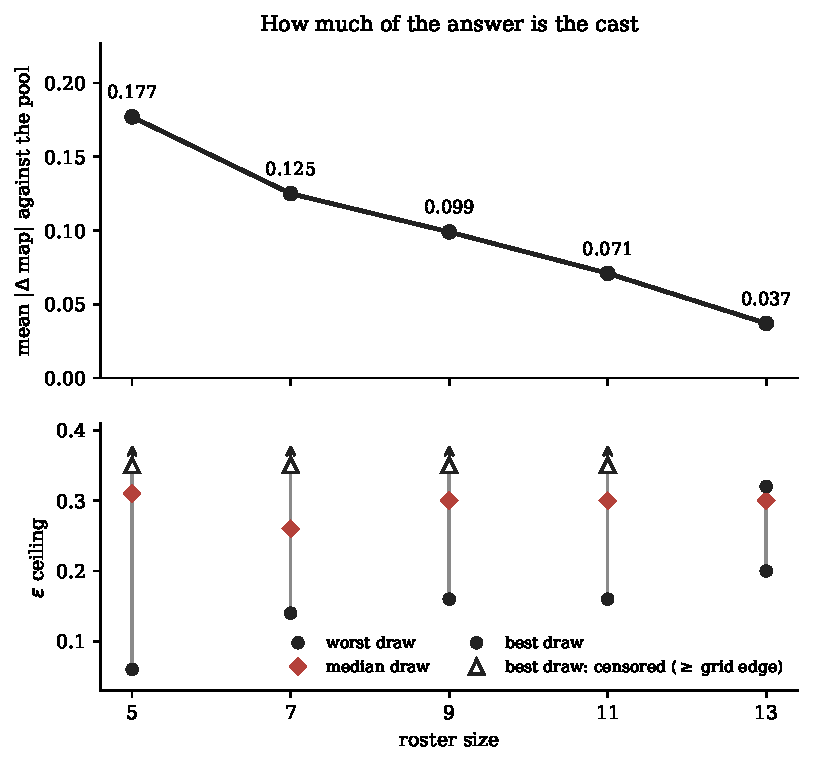
\includegraphics[width=0.86\linewidth]{fig5_sensitivity.pdf}
  \caption{How much of the answer is the cast. Upper panel: the mean absolute
  difference between a drawn sub-roster's map and the pool's, against roster
  size. Lower panel: the spread of $\eps$ ceilings at each size. Open upward
  triangles mark censored values --- rosters still cooperating in the last
  column of the grid, for which the measurement is a lower bound and not a
  location. \source{results/fig5\_sensitivity.csv}}
  \label{fig:sensitivity}
\end{figure}

\subsection{Influence}
\label{sec:influence}
% TODO

\begin{figure}[t]
  \centering
  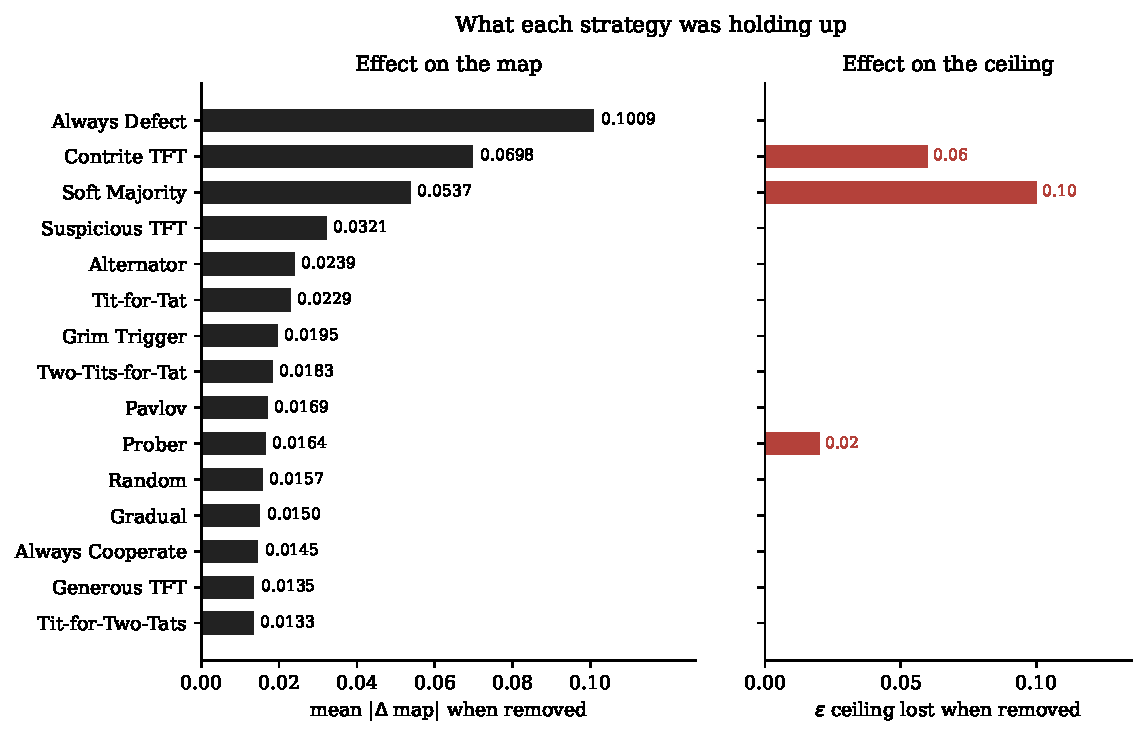
\includegraphics[width=\linewidth]{fig4_influence.pdf}
  \caption{Each strategy removed in turn, and the map re-derived from the
  remaining submatrix. Left: how far the map moves. Right: how much $\eps$
  ceiling is lost. The two rank differently, and the difference is the point
  --- the strategy that moves the map most costs no ceiling at all.
  \source{results/fig4\_influence.csv}}
  \label{fig:influence}
\end{figure}

\subsection{Three ways of surviving error}
\label{sec:mechanisms}
% TODO

\section{Corrections}
\label{sec:corrections}
% TODO

\section{Discussion}
\label{sec:discussion}
% TODO

\section{Limitations}
\label{sec:limitations}
% TODO

\section{Conclusion}
\label{sec:conclusion}
% TODO

\appendix

\section{Reproducibility}
\label{sec:repro}
% TODO

\section{Decision log}
\label{sec:decisions}
% TODO

% The section bodies are empty, so nothing cites anything yet and the
% bibliography would come out blank - which would also mean the bibliography
% pass had never actually been exercised by a build. \nocite{*} typesets every
% entry, so `python build_report.py` is a real test of references.bib. Remove
% it once the prose carries its own citations.
\nocite{*}
\bibliography{references}

\end{document}
